
\documentclass[article,11pt]{article}

\usepackage{fullpage}
\usepackage{url}
\usepackage[english]{babel}
\usepackage[utf8]{inputenc}
\usepackage{amsmath}
\usepackage{bm, amssymb}
\usepackage{graphicx}
\graphicspath{ {/} }
\renewcommand*{\thesection}{Problem~\arabic{section}:}
\renewcommand{\labelenumi}{(\alph{enumi})}
\newcommand{\Tt}[0]{\boldsymbol{\theta}}
\newcommand{\XX}[0]{{\cal X}}
\newcommand{\ZZ}[0]{{\cal Z}}
\newcommand{\vx}[0]{{\bf x}}
\newcommand{\vv}[0]{{\bf v}}
\newcommand{\vu}[0]{{\bf u}}
\newcommand{\vs}[0]{{\bf s}}
\newcommand{\vm}[0]{{\bf m}}
\newcommand{\mX}[0]{{\bf X}}
\newcommand{\vw}[0]{{\bf w}}
\newcommand{\D}[0]{{\mathcal{D}}}
\newcommand{\mP}{\mathbf{P}}
\newcommand{\E}[0]{{\mathbb{E}}}
\newcommand{\vy}[0]{{\bf y}}
\newcommand{\vb}[0]{{\bf b}}
\newcommand{\vr}[0]{{\bf r}}
\newcommand{\vz}[0]{{\bf z}}
\newcommand{\N}[0]{{\mathcal{N}}}
\newcommand{\vc}[0]{{\bf c}}
\newcommand{\norm}[1]{\Vert  {#1} \Vert}
%\newcommand{\XX}[0]{X}
%\newcommand{\ZZ}[0]{Z}
\newcommand{\bmx}[0]{\begin{bmatrix}}
\newcommand{\emx}[0]{\end{bmatrix}}
%\newcommand{\norm}[1]{\lVert#1\rVert}
\newcommand{\T}[0]{\text{T}}
\DeclareMathOperator*{\rank}{rank}
\newcommand\defeq{:=}
\newcommand\eigvecS{\hat{\mathbf{u}}} 
\newcommand\eigvecCov{\mathbf{u}} 
\newcommand{\featuredim}{d}
\newcommand{\samplesize}{N}
\newcommand{\sampleidx}{i} 
\newcommand{\target}{y}
\newcommand{\error}{E}
\newcommand\dataset{\mathbb{X}}
\newcommand{\inspace}{\mathcal{X}}
\newcommand{\sigmoid}{\sigma}
\newcommand{\outspace}{\mathcal{Y}}
\newcommand{\hypospace}{\mathcal{H}}
\newcommand{\emperror}{\mathcal{E}}
\newcommand{\generror}{\mathcal{E}}
\DeclareMathOperator{\supp}{supp}
%\newcommand{\loss}[3]{L({#1},{#2},{#3})} 
\newcommand{\loss}[2]{L({#1},{#2})} 
\newcommand{\determinant}[1]{{\rm det}({#1})} 
\newcommand{\prob}[1]{P({#1})} 
\newcommand{\pdf}[1]{p({#1})} 
\def \expect {\mathsf{E} }
\DeclareMathOperator*{\argmax}{argmax}
\DeclareMathOperator*{\argmin}{argmin}
%\def \prob {{\rm P} }



\newcommand{\coefflen}{p}
\setlength{\textheight}{53\baselineskip} % number of lines per side
\setlength{\textheight}{51\baselineskip} % number of lines per side
\textwidth176mm
\oddsidemargin=-8mm
\evensidemargin=-8mm  %Rand auf geraden Seiten ist etwa 24.5mm
\topmargin=-12mm
\unitlength1mm
%\pagestyle{headings}
%\renewcommand{\baselinestretch}{1.5}  % 1.1 fache des normalen Zeilenabstandes
\renewcommand{\textfraction}{0.0}      % 10% einer Seite mit Gleitobjekt muß Text sein
\addtolength{\hoffset}{-0.5cm}
\addtolength{\voffset}{0.3cm}
\addtolength{\topmargin}{-0.5cm}
\addtolength{\textwidth}{1cm}
\addtolength{\textheight}{1cm}

\title{CS-E3210- Machine Learning Basic Principles \\ Home Assignment 2 - ``Regression''}
\begin{document}
\date{}
\maketitle

Your solutions to the following problems should be submitted as one single pdf which does not contain 
any personal information (student ID or name). The only rule for the layout of your submission is that for each 
problem there has to be exactly one separate page containing the answer to the problem. You are welcome to use the \LaTeX-file underlying this pdf, 
available under \url{https://version.aalto.fi/gitlab/junga1/MLBP2017Public}, and fill in your solutions there. 

\newpage
\section{``Plain Vanilla'' Linear Regression}
\label{problem_1}

Consider a dataset $\dataset$ which is constituted of $\samplesize\!=\!10$ webcam snapshots with filename 
``MontBlanc*$\sampleidx$*.png'', $\sampleidx=1,\ldots,\samplesize$, available in the folder ``Webcam'' at \url{https://version.aalto.fi/gitlab/junga1/MLBP2017Public}. 
Determine for each snapshot the feature vector $\vx^{(\sampleidx)}=(x_{\rm g}^{(\sampleidx)},1)^{T} \in \inspace (= \mathbb{R}^{2})$ with the normalized (by the number of image pixels) greenness $x_{\rm g}^{(\sampleidx)}$. 
Moreover, determine for each snapshot the label $y^{(\sampleidx)} \in \outspace (=\mathbb{R})$ given by the duration (in minutes) after 07:00 am, at which the picture has been taken. 
We want to find (learn) a predictor $h(\cdot): \inspace \rightarrow \outspace$ which allows to predict the value of $y^{(\sampleidx)}$ directly from 
the value of the feature $x_{\rm g}^{(\sampleidx)}$. To this end we consider only predictors belonging to the hypothesis space 
$\hypospace = \{h^{(\vw)}(\vx) = \vw^{T} \vx \mbox{ for some } \vw \in \mathbb{R}^{2}\}$. 
The quality of a particular predictor is measured by the mean squared error 
\vspace*{-3mm}
\begin{equation} \label{eq:1}
 \emperror(h(\cdot) | \dataset) \defeq  \frac{1}{\samplesize}\sum^{\samplesize}_{\sampleidx=1}(y^{(\sampleidx)} - h(\vx^{(\sampleidx)}))^2= \frac{1}{\samplesize}\sum^{\samplesize}_{\sampleidx=1}(y^{(\sampleidx)} - \vw^{T} \vx^{(\sampleidx)})^2.
\vspace*{-2mm}
\end{equation} 
Note that the mean squared error is nothing but the empirical risk obtained when using the squared error loss $\loss{(\vx,y)}{h(\cdot)} = (y - h(\vx))^{2}$ (cf.\ Lecture 2). 

The optimal predictor $h_{\rm opt}(\cdot)$ is then
\vspace*{-3mm}
\begin{equation}
\label{equ_opt_problem_hypo}
h_{\rm opt}(\cdot)  = \argmin_{h(\cdot) \in \hypospace}  \emperror(h(\cdot) | \dataset). 
\vspace*{-2mm}
\end{equation}
We can rewrite this optimization problem in a fully equivalent manner in terms of the weight 
$\vw$ representing a particular predictor $h^{(\vw)}(\cdot) \in \hypospace$ as 
\vspace*{-5mm}
\begin{equation}
\label{equ_opt_problem_weight}
\vw_{\rm opt} = \argmin_{\vw \in \mathbb{R}^{2}}   \frac{1}{\samplesize}\sum^{\samplesize}_{\sampleidx=1}(y^{(\sampleidx)} - \vw^{T} \vx^{(\sampleidx)})^2. 
\vspace{-3mm}
\end{equation}
As can be verified easily, the optimal predictor $h_{\rm opt}(\cdot)$ (cf.\ \eqref{equ_opt_problem_hypo}) is obtained as 
$h_{\rm opt}(\cdot) = h^{(\vw_{\rm opt})}(\cdot)$ with the optimal weight vector $\vw_{\rm opt}$ (cf.\ \eqref{equ_opt_problem_weight}).

Can you find a closed-form expression for the optimal weight $\vw_{\rm opt}$ (cf.\ \eqref{equ_opt_problem_weight}) in terms of the vectors 
$\vx = (x_{\rm g}^{(1)},\ldots,x_{\rm g}^{(\samplesize)})^{T} \in \mathbb{R}^{\samplesize}$, and $\vy = (y^{(1)}, \ldots,y^{(\samplesize)})^{T}\in \mathbb{R}^{\samplesize}$?

\noindent{\bf Answer.}
% VASTAUS ALKAA
\vspace{3mm}

A optimized and closed-form expression for $w_{opt}$ is achieved by minimizing $\mathcal {E}(h(\cdot)|\mathbb{X})$, by solving where its gradient is 0. The below equations are based on what is found in chapter 5.1.4. of the Deep Learning book.  

$$
\begin{gathered}
\frac{\delta \mathcal {E}(h(\cdot)|\mathbb{X})}{\delta w} = 0 \Leftrightarrow \bigtriangledown_w [\frac{1}{N}(y-Xw)]= 0 \Leftrightarrow \bigtriangledown_w[y^T y - w^T X^T y - y^T Xw + w^T X^T Xw] = 0 \\ \Leftrightarrow -X^T y + X^T Xw = 0 \Leftrightarrow (X^T X)w = X^T y \Leftrightarrow w = (X^T X)^{-1} X^T y 
\end{gathered}
$$

Inserting the values of the images (visible in screen cap below) into the calculation gives us that for this case 
$$
\begin{gathered}
\hat{w} = w_{opt} = (X^T X)^{-1} X^Ty \\ = [-439.99985992, 6.148722404]
\end{gathered}
$$

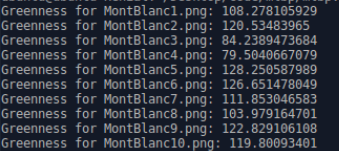
\includegraphics{greenness}

\vspace{3mm}
% VASTAUS PÄÄTTYY
\newpage
\section{``Plain Vanilla'' Linear Regression - Figure}
\label{problem_1}

Reconsider the setup of Problem 1 and generate a plot with horizontal (vertical) axis representing greenness $x_{\rm g}$ (label $y$), which depicts the optimal predictor 
$h_{\rm opt}(\cdot)$ (cf.\ \eqref{equ_opt_problem_hypo}) and also contains the data points $(x_{\rm g}^{(\sampleidx)},y^{(\sampleidx)})$ for $\sampleidx=1,\ldots,\samplesize$. 
Do you consider it feasible to predict the daytime accurately from the greenness?

\noindent{\bf Answer.}
%VASTAUS 2 ALKAA
\vspace{3mm}
\\ Judging by the graph (found below), it seems pretty feasible on first look to predict the time of day from greenness, however looking at mean squared error for the case gives us:

$$
\begin{gathered}
\mathcal {E}(h(\cdot)|\mathbb{X})= \frac{1}{N} \sum_{i=1}^{N} (y^{(i)} - h(x^{(i)}))^2 = \frac{1}{N} \sum_{i=1}^{N} (y^{(i)} - w^T x^{(i)} )^2 = 783.424339374

\end{gathered}
$$

which does not seem not very accurate in the end.

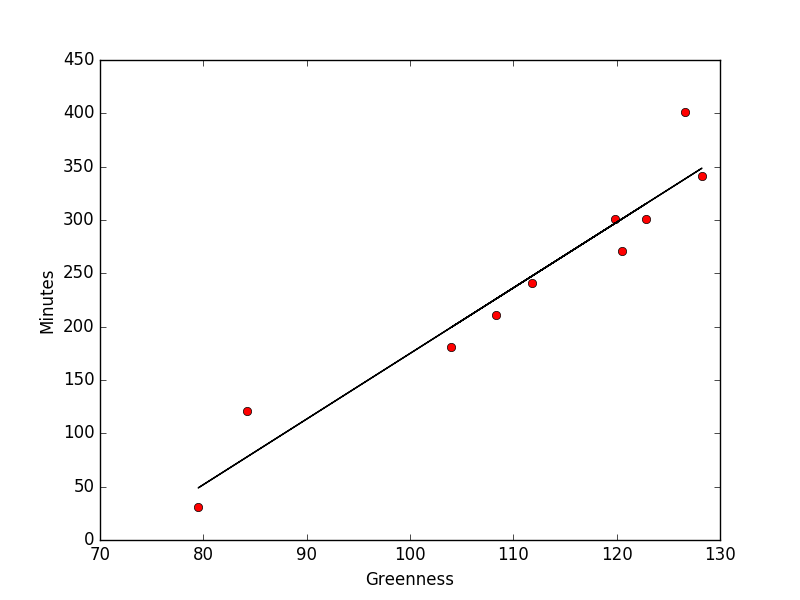
\includegraphics{figure_2}
%VASTAUS 2 PÄÄTTYY
\vspace{3mm}
\newpage


\newpage

\section{Regularized Linear Regression}
We consider again the regression problem of Problem 1, i.e., predicting the daytime of a webcam snapshot based on 
the feature vector $(x_{\rm g},1)^{T}$. The prediction is of the form $h^{(\vw)}(\vx) = \vw^{T} \vx$ 
with some weight vector $\vw \in \mathbb{R}^{2}$. Assume that we only have snapshots which are taken within $7$ hours after 07:00 am, i.e.,the 
value of the label $y$ cannot exceed $420$. Therefore, it makes sense to somehow constraint the norm of the weight vector $\vw$ to 
exclude unreasonable predictions. To this end, we augment the mean squared error \eqref{eq:1} with the ``regularization term'' $\lambda \| \vw\|^{2} $ 
which penalizes ``atypical'' values for the weight vector. The optimal predictor $h_{\rm opt}(\cdot)$ using this regularization term is then given by 
\begin{equation}
\label{equ_opt_problem_hypo_r}
h_{\rm opt,r}(\cdot)  = \argmin_{h^{(\mathbf{w})}(\cdot) \in \hypospace} \big(  \emperror(h^{(\mathbf{w})}(\cdot) | \dataset)+ \lambda \| \vw \|^{2} \big). 
\vspace*{-2mm}
\end{equation}
Again, we can rewrite this optimization problem in a fully equivalent manner in terms of the weight 
$\vw$ representing a particular predictor $h^{(\vw)}(\cdot) \in \hypospace$ as 
\vspace*{-5mm}
\begin{equation}
\label{equ_opt_problem_weight_r}
\vw_{\rm opt,r} = \argmin_{\vw \in \mathbb{R}^{2}}   \frac{1}{\samplesize}\sum^{\samplesize}_{\sampleidx=1}(y^{(\sampleidx)} - \vw^{T} \vx^{(\sampleidx)})^2 + \lambda \| \vw \|^{2}. 
\vspace{-3mm}
\end{equation}
As can be verified easily, the optimal predictor $h_{\rm opt,r}(\cdot) \in \hypospace$ solving \eqref{equ_opt_problem_hypo} is obtained as 
$h_{\rm opt,r}(\cdot) = h^{(\vw_{\rm opt,r})}(\cdot)$ with the optimal weight vector $\vw_{\rm opt,r}$ which is the solution of \eqref{equ_opt_problem_weight}.
Can you find a closed-form solution for the optimal weight $\vw_{\rm opt,r}$ (cf.\ \eqref{equ_opt_problem_weight}) in terms of the vectors 
$\vx = (x_{\rm g}^{(1)},\ldots,x_{\rm g}^{(\samplesize)})^{T} \in \mathbb{R}^{\samplesize}$, and $\vy = (y^{(1)}, \ldots,y^{(\samplesize)})^{T}\in \mathbb{R}^{\samplesize}$ and $\lambda$?
\noindent {\bf Answer:}

%VASTAUS 3 ALKAA
\vspace{3mm}
\\ A closed-form solution can be achieved with the following, providign an optimal $w_{opt}$:

$$
\begin{gathered}
\frac{\mathcal {E}(h(\cdot)|\mathbb{X}) + \lambda ||w||^2}{\delta w}= 0 \Leftrightarrow \bigtriangledown_w [\frac{1}{N}(y - Xw)^T (y - Xw) + N\lambda w^T w] = 0 \\
\Leftrightarrow \bigtriangledown_w [y^y - w^TX^Ty - y^T Xw + w^T X^T Xw + N \lambda w^T w] = 0 \\
\Leftrightarrow -X^T y + X^TXw+N \lambdaw = \Leftrightarrow (X^T X + N \lambda I) w = X^T y \\
\Leftrightarrow w = (X^T X + N \lambda I)^{-1} X^T y

\end{gathered}
$$

Based on the above, the optimal paramater is: $ \hat{w} = w_{opt,r} = (X^T X + N \lambda I)^{-1} X^T y  $

%VASTAUS 3 PÄÄTTYY

\newpage
\section{Regularized Linear Regression - Figure}
Reconsider the setup of Problem 3 and generate a plot with horizontal (vertical) axis representing greenness $x_{\rm g}$ (label $y$) 
which contains the data points $(x_{\rm g}^{(\sampleidx)},y^{(\sampleidx)})$, for $\sampleidx=1,\ldots,\samplesize$, and 
depicts the optimal predictor $h_{\rm opt,r}(\cdot)$ (cf.\ \eqref{equ_opt_problem_hypo_r}) for the two particular choices $\lambda=2$ and $\lambda=5$. 
Which choice for $\lambda$ seems to be better for the given task? 

\noindent {\bf Answer:}
%VASTAUS 4 ALKAA
\vspace{3mm}
\\ A closed-form solution can be achieved with the following, providign an optimal $w_{opt}$:

\newpage


\section{Gradient Descent for Linear Regression}
Consider the same dataset as in Problem 1, i.e., the set of $\samplesize=10$ webcam snapshots which are labeled by the daytime $y^{(\sampleidx)}$ 
when the image has been taken. As in Problem 1, we are interested in predicting the daytime directly from the image. However, by contrast 
to Problem 1 where we only used the greenness $x_{\rm g}^{(\sampleidx)}$ of the $\sampleidx$-th image, we know use the green intensity 
values for the upper-left area consisting of $100 \times 100$ pixels, 
which we stack into the feature vector $\vx^{(\sampleidx)} \in \mathbb{R}^{d}$. What is the length $d$ of the feature vector $\vx^{(\sampleidx)}$ here? 
Based on the feature vector, we predict the daytime by a predictor of the form $h^{(\vw)}(\vx) = \vw^{T} \vx$ with some weight vector $\vw \in \mathbb{R}^{d}$. 
The optimal predictor is obtained by solving an empirical risk minimization problem of the form \eqref{equ_opt_problem_hypo}, 
or directly in terms of the weight vector, \eqref{equ_opt_problem_weight}. This minimization problems can be solved by a simple but powerful iterative method 
known as gradient descent (GD): 
\vspace*{-2mm}
\begin{equation}
\label{equ_GD_iteration}
    \vw^{(k+1)} = \vw^{(k)} - \alpha \nabla f(\vw^{(k)}) 
 \vspace*{-2mm}
\end{equation}
with some positive step size $\alpha >0$ and the mean-squared error cost function (cf.\ \eqref{eq:1}) 
\vspace*{-2mm}
\begin{equation} 
f(\vw) \defeq \emperror(h^{(\vw)}|\dataset) \stackrel{\eqref{eq:1}}{=} \frac{1}{\samplesize}\sum^{\samplesize}_{\sampleidx=1}(y^{(\sampleidx)} - \vw^{T} \vx^{(\sampleidx)})^2. \nonumber
\vspace*{-2mm}
\end{equation} 
In order to implement the GD iterations \eqref{equ_GD_iteration}, we need to compute the gradient $\nabla f(\vw)$. 
Can you find a simple closed-form expression for the gradient of $f(\mathbf{w})$ at a particular weight vector $\vw$?

The performance of GD depends crucially on the particular value chosen for the step size $\alpha$ in \eqref{equ_GD_iteration}. 
Try out different choices for the step size $\alpha$ and, for each choice plot the evolution of the empirical risk 
$\emperror(h^{(\vw^{(k)})}| \dataset)$ as a function of iteration number $k$ into one single figure. 
Use the initialization $\vw^{(0)} = \mathbf{0}$ for the GD iterations for each run. 

Another crucial issue when using GD is the question of when to stop iterating \eqref{equ_GD_iteration}. Can you 
state a few stopping criteria that indicate when it would be reasonable to stop iterating \eqref{equ_GD_iteration}?

\noindent {\bf Answer:}


\newpage
\section{Gradient Descent for Regularized Linear Regression}
Redo Problem 5 by using regularized linear regression (cf.\ Problem 3) instead of linear regression. 

\noindent {\bf Answer:}

\newpage
\section{Kernel Regression}
Consider the data set of Problem 1, i.e., the set of $\samplesize=10$ webcam snapshots. Let us now represent each webcam snapshot by 
the single feature $x^{(\sampleidx)} = x_{\rm g}^{(\sampleidx)}$, i.e., the total greenness of the $\sampleidx$th snapshot. We aim 
at predicting the daytime $y^{(\sampleidx)}$ based solely on the greenness. In contrast to Problem 1 and Problem 2 we will now 
use a different hypothesis space of predictors. In particular, we only consider predictors out of the hypothesis space
\begin{equation}
\hypospace = \bigg\{h^{(\sigma)}(\cdot): \mathbb{R} \rightarrow \mathbb{R}: h^{(\sigma)} (x) = \sum_{\sampleidx=1}^{\samplesize} y^{(\sampleidx)} \frac{K_\sigma(x,x^{(\sampleidx)})}{\sum_{l=1}^{\samplesize} K_\sigma (x,x^{(l)})} \bigg\}
\end{equation}
with the ``kernel''  
\begin{equation}
K_\sigma(x, x^{(\sampleidx)}) = \exp \Bigg( -\frac{1}{2} \frac{(x-x^{(\sampleidx)})^2 }{\sigma^2} \Bigg).
\end{equation}
Try out predicting the daytime $y^{(\sampleidx)}$ using the greenness $x_{\rm g}^{(\sampleidx)}$ using a predictor $h^{(\sigma)}(\cdot) \in \hypospace$ using the 
choices $\sigma \in \{1,5,10\}$. Generate a plot with horizontal (vertical) axis representing greenness $x_{\rm g}$ (label $y$), which depicts the predictor 
$h^{(\sigma)}(\cdot)$ for $\sigma \in \{1,5,10\}$ and also contains the data points $(x_{\rm g}^{(\sampleidx)},y^{(\sampleidx)})$.
Which choice for $\sigma$ achieves the lowest mean squared error $\emperror(h^{(\sigma)}| \dataset)$ (cf. \eqref{eq:1}) ?

\noindent {\bf Answer:}

\newpage
\section{Linear Regression using Feature Maps}
Consider a regression problem, where we aim at predicting the value of a real-valued label or target or output variable $y \in \mathbb{R}$ of a data point 
based on a single feature $x \in \mathbb{R}$ of this data point. We assume that there is some true underlying functional relationship between 
feature $x$ and output $y$, i.e., $y =h^{*}(x)$ with some unknown function (hypothesis). All we know about this true underlying functional relationship is 
that 
\vspace*{-2mm}
\begin{equation}
\label{equ_properties_hypo}
h^{*}(x) = 0 \mbox{ for any } x \notin [0,10]  \mbox{, and } |h^{*}(x') -h^{*}(x'')| \leq 10^{-3} |x'-x''| \mbox{ for any } x',x'' \in[0,10]. 
\vspace*{-2mm}
\end{equation}
We apply then a feature map ${\bm \phi}: \mathbb{R} \rightarrow \mathbb{R}^{n}$, with some suitable chosen dimension $n$, which transforms 
the original feature $x$ into a modified feature vector ${\bm \phi}(x)=(\phi_{1}(x),\ldots,\phi_{n}(x))^{T}$. We use the transformed features 
${\bm \phi}(x)$ to predict the label $y$ using the predictor $h^{(\mathbf{w})}(x) = \mathbf{w}^{T} {\bm \phi}(x)$ with some weight vector $\mathbf{w}\in \mathbb{R}^{n}$. 
Note that the so defined predictor $h^{(\mathbf{w})}$ is linear only w.r.t.\ the high-dimensional features ${\bm \phi}(x)$, but typically 
a non-linear function of the original feature $x$. Is there a feature map ${\bm \phi}$ which allows to approximate the true hypothesis $h^{*}(\cdot)$ (
which satisfies \eqref{equ_properties_hypo}) by some predictor $h^{(\mathbf{w}_{0})}(x) =  \mathbf{w}_{0}^{T} {\bm \phi}(x)$ with a suitably chosen weight $\mathbf{w}_{0}$?
In particular, is there a feature map ${\bm \phi}$ and weight vector $\mathbf{w}_{0} \in \mathbb{R}^{n}$ such that $|h^{(\mathbf{w}_{0})}(x) - h^{*}(x)| \leq 10^{-3}$ for all $x \in \mathbb{R}$?

\noindent {\bf Answer:}
\end{document}